% !TEX TS-program = pdflatex
% !TEX encoding = UTF-8 Unicode

% This is a simple template for a LaTeX document using the "article" class.
% See "book", "report", "letter" for other types of document.

\documentclass[11pt]{article} % use larger type; default would be 10pt

\usepackage[utf8]{inputenc} % set input encoding (not needed with XeLaTeX)

%%% PAGE DIMENSIONS
\usepackage{geometry} % to change the page dimensions
\geometry{a4paper} % or letterpaper (US) or a5paper or....
\geometry{margin=1in} 
\usepackage{graphicx} % support the \includegraphics command and options

\usepackage{amssymb}
\usepackage{amsmath}
%%% PACKAGES
\usepackage{booktabs} % for much better looking tables
\usepackage{array} % for better arrays (eg matrices) in maths
\usepackage{paralist} % very flexible & customisable lists (eg. enumerate/itemize, etc.)
\usepackage{verbatim} % adds environment for commenting out blocks of text & for better verbatim
\usepackage{subfig} % make it possible to include more than one captioned figure/table in a single float
% These packages are all incorporated in the memoir class to one degree or another...

%%% HEADERS & FOOTERS
\usepackage{fancyhdr} % This should be set AFTER setting up the page geometry
\pagestyle{fancy} % options: empty , plain , fancy
\renewcommand{\headrulewidth}{0pt} % customise the layout...
\lhead{}\chead{}\rhead{}
\lfoot{}\cfoot{\thepage}\rfoot{}

%%% SECTION TITLE APPEARANCE
\usepackage{sectsty}
\allsectionsfont{\sffamily\mdseries\upshape} % (See the fntguide.pdf for font help)
% (This matches ConTeXt defaults)

%%% ToC (table of contents) APPEARANCE
\usepackage[nottoc,notlof,notlot]{tocbibind} % Put the bibliography in the ToC
\usepackage[titles,subfigure]{tocloft} % Alter the style of the Table of Contents
\renewcommand{\cftsecfont}{\rmfamily\mdseries\upshape}
\renewcommand{\cftsecpagefont}{\rmfamily\mdseries\upshape} % No bold!
\usepackage{graphicx}
\graphicspath{ {./pings/} }

\usepackage{amsmath}
\DeclareMathOperator*{\argmax}{arg\,max}
\DeclareMathOperator*{\argmin}{arg\,min}

\newcount\colveccount
\newcommand*\colvec[1]{
        \global\colveccount#1
        \begin{pmatrix}
        \colvecnext
}
\def\colvecnext#1{
        #1
        \global\advance\colveccount-1
        \ifnum\colveccount>0
                \\
                \expandafter\colvecnext
        \else
                \end{pmatrix}
        \fi
}

%%% END Article customizations

%%% The "real" document content comes below...

\title{Macro PS3}
\author{Michael B. Nattinger\footnote{I worked on this assignment with my study group: Alex von Hafften, Andrew Smith, and Ryan Mather. I have also discussed problem(s) with Emily Case, Sarah Bass, Katherine Kwok, and Danny Edgel.}}

%\date{} % Activate to display a given date or no date (if empty),
         % otherwise the current date is printed 

\begin{document}
\maketitle
\section{Question 1}
I have pulled the relevant data off of FRED. Data series are plotted below. Note that Employment data is listed on FRED at a monthly frequency, so I converted to quarterly by averaging within the quarter (as opposed to using end-of-quarter employment numbers).

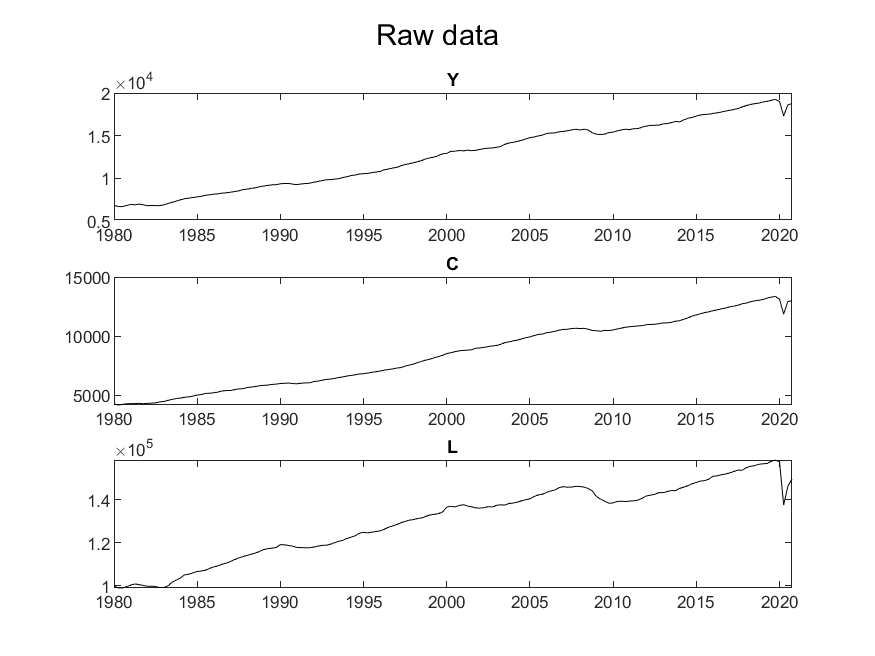
\includegraphics{raw}

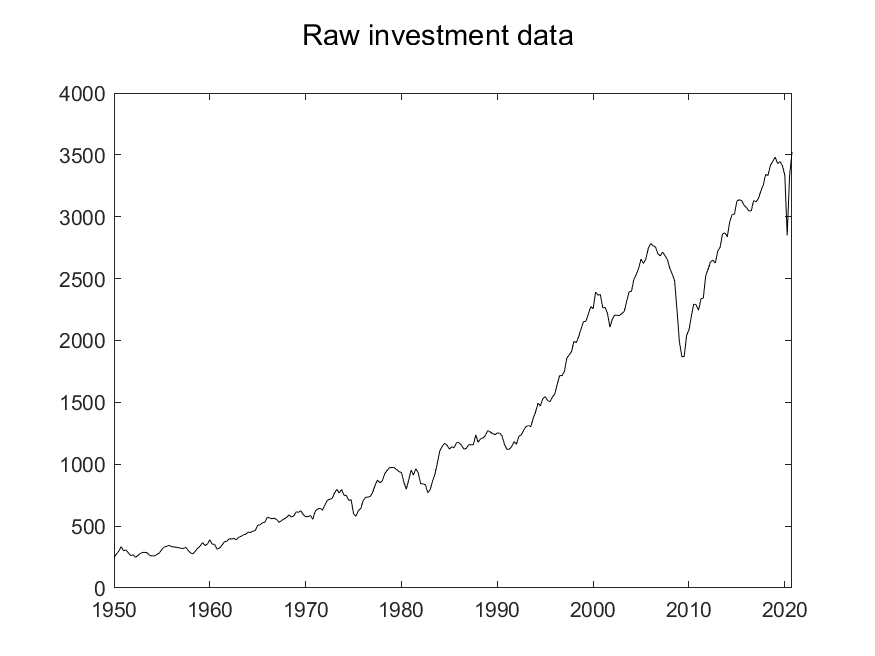
\includegraphics{rawi}

\section{Question 2}

We next log the data, and extract an HP filter (smoothing parameter 1600) from the logged data. We plot below.

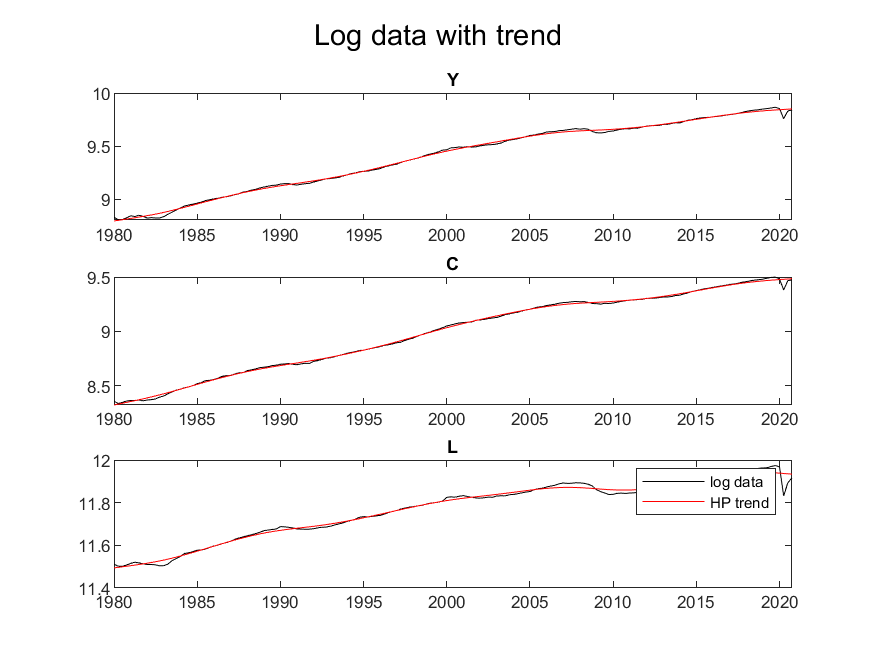
\includegraphics{log}

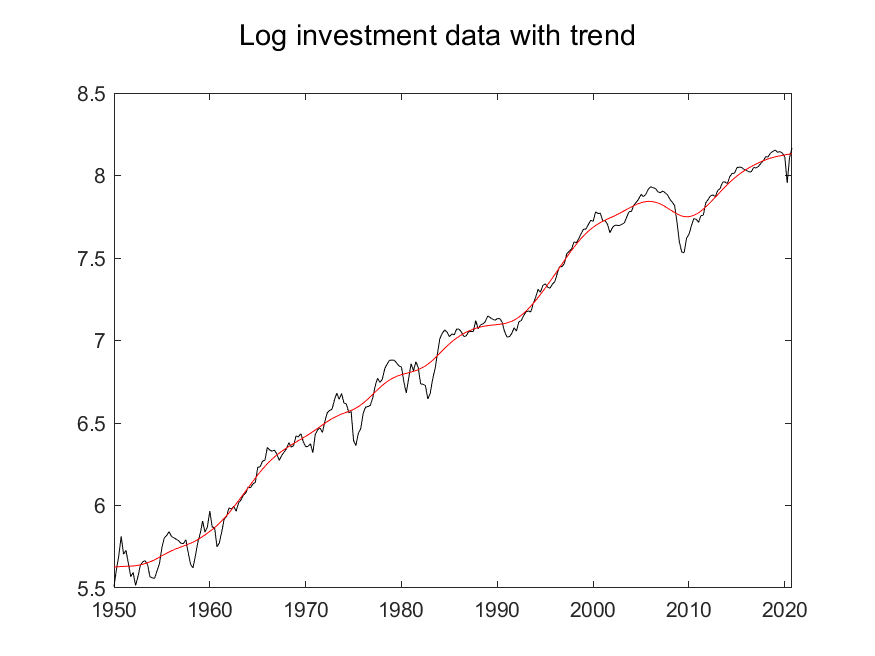
\includegraphics{logi}

The detrended data is below.

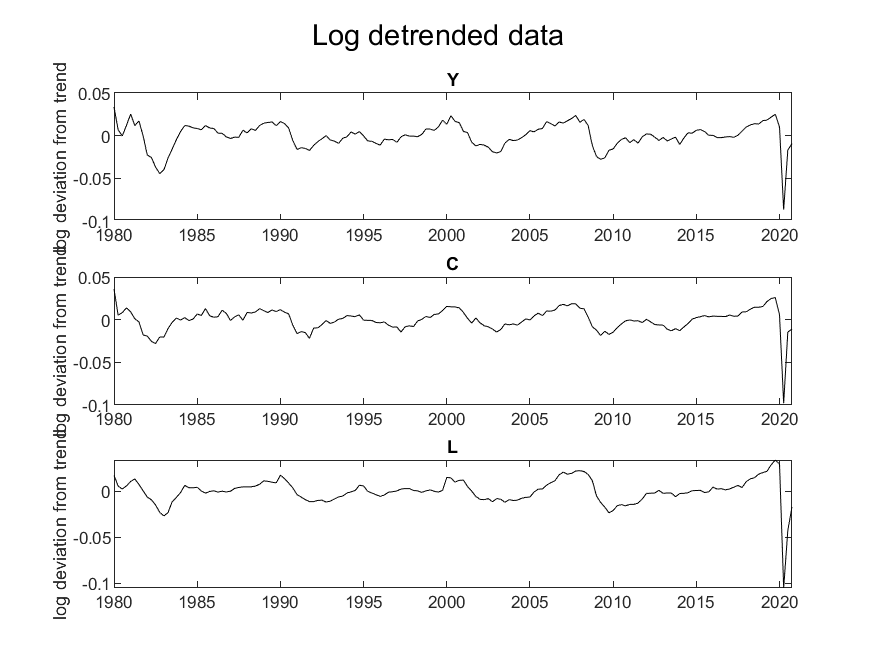
\includegraphics{det}

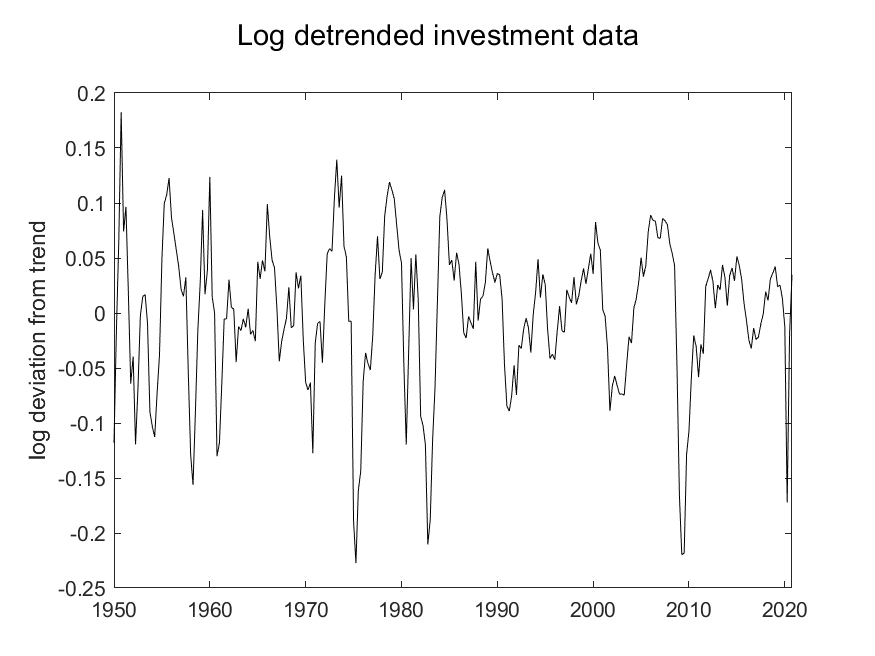
\includegraphics{deti}

\section{Question 3}

Our capital law of motion can be log linearized as such:

\begin{align*}
K_{t+1} &= (1-\delta) K_{t} + I_{t}\\
\bar{I} &= \delta \bar{K}\\
\bar{K}(1+k_{t+1}) &= \bar{K}(1-\delta)(1+k_t) + \bar{I}(1+i_t)\\
\bar{K}k_{t+1} &= \bar{K}(1-\delta)k_t + \bar{I}i_t\\
k_{t+1} &= (1-\delta)k_t + \delta i_t.
\end{align*}

We can iteratively decompose the law of motion as follows:
\begin{align*}
k_{t+1} &= (1-\delta)k_t + \delta i_t\\
&= \delta i_t + (1-\delta)((1-\delta)k_{t-1} + \delta i_{t-1})\\
&= \delta (i_t + (1-\delta) i_{t-1}) + (1-\delta)^2((1-\delta)k_{t-2} + \delta i_{t-2})\\
&= \delta \sum_{j=0}^J(1-\delta)^j i_{t-j} +(1-\delta)^{J+1} k_{t-J}
\end{align*}
We have 30 years of quarterly investment data before our capital series starts, so 120 observations. We do not know our capital deviation from trend in 1950, but notice that this term has very little impact on our capital deviation from trend in 1980:
\begin{align*}
k_{1980Q1} &= \delta \sum_{j=0}^{119}(1-\delta)^j i_{1979Q4-j} +(1-\delta)^{120} k_{1950Q1}
\end{align*}

Our capital deviations from steady state are already very small to begin with, and the $k_{1950Q1}$ term above is multiplied by $(1-\delta)^{120}.$ Given our parameterization of $\delta$, $0.025$, $(1-\delta)^{120} = 0.048.$ This means that our capital level in the first quarter of 1950 accounts for less than $5$ percent of our capital level at the beginning of $1980$, and even less so as we get later in the sample. As we were already approximating cross-terms in the log linearization as being approximately zero, this term is on the same order of magnitude and can, therefore, be safely approximated to zero.

I implemented the perpetual inventory method to estimate the capital stock over 1980 - 2020. Results are below:

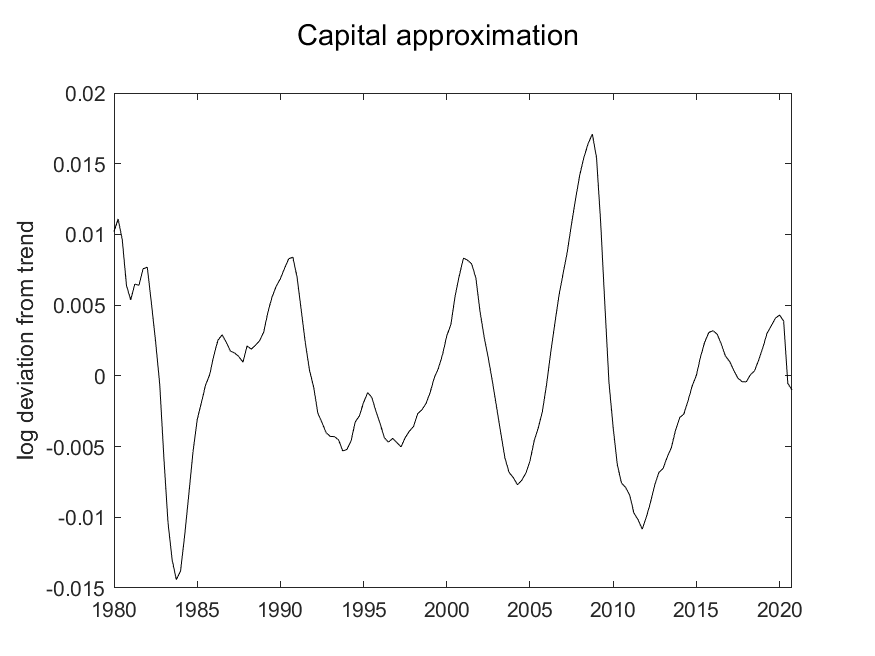
\includegraphics{detk}

\section{Question 4}
Our equilibrium consists of the following equations:
\begin{align}
Y_{t} &= A_tK_t^{\alpha}L_t^{1-\alpha} \label{F}\\
Y_{t} &= C_{t} + I_{t} + G_{t} \label{Y}\\
L_{t}^{\phi}C_t^{\sigma} &= (1-\tau_{L,t})A_t(1-\alpha) K_t^{\alpha}L_t^{-\alpha} \label{L}\\
C_t^{-\sigma}(1+\tau_{I,t}) &= \beta E_t[C_{t+1}^{-\sigma}[A_{t+1}\alpha K_{t+1}^{\alpha-1}L_{t+1}^{1-\alpha} + (1-\delta)(1+\tau_{I,t+1})]] \label{EE}
\end{align}

We will proceed by linearizing our conditions. First, the production function (\ref{F}):
\begin{align}
y_t &= a_t + \alpha k_t + (1-\alpha) l_t. \label{f}
\end{align}
Next, our market clearing condition (\ref{Y}):
\begin{align}
y_t &= \frac{\bar{C}}{\bar{Y}}c_t + \frac{\bar{I}}{\bar{Y}} i_t + \frac{\bar{G}}{\bar{Y}} g_t. \label{y}
\end{align}
Then, our labor supply equation (\ref{L}) (note that $\bar{\tau_{I}},\bar{\tau_{L}}$ equal 0 so $\tau_{I,t},\tau_{L,t}$ are linearized and not log linearized):

\begin{align*}
\bar{L}^{\phi}\bar{C}^{\sigma}(1+\sigma c_t + \phi l_t) &= \bar{X} \bar{A}(1-\alpha) \bar{K}^{\alpha}\bar{L}^{-\alpha}(1+x_t + a_t + \alpha k_t - \alpha l_t) \\
\sigma c_t + \phi l_t &= x_t + a_t + \alpha k_t - \alpha l_t\\
\bar{X}(1+x_t) &= 1-\hat{\tau}_{L,t}\\
x_t &=-\hat{\tau}_{L,t}
\end{align*}

\begin{align}
\phi l_t + \sigma c_t &= -\hat{\tau}_{L,t} + a_t +\alpha k_t -\alpha l_t. \label{l}
\end{align}
Finally, we linearize our Euler equation:

\begin{align*}
\bar{C}(1- \sigma c_t )\bar{Y}(1+y_t) &= \beta E_t[\bar{C}(1- \sigma c_{t+1})\bar{X}(1+x_{t+1})]\\
\sigma(E_t[c_{t+1}] - c_t) + y_t &= E_t[x_{t+1}], \\
Y_t &= 1+\tau_{I,t}\\
\bar{Y}(1+y_t) &= 1 + \hat{\tau}_{I,t}\\
y_t &= \hat{\tau}_{I,t}\\
\bar{X}(1+x_t) &= \bar{A}(1+a_{t})\alpha \bar{K}^{\alpha-1}(1+(\alpha-1)k_{t}) \bar{L}_{t}^{1-\alpha}(1+(1-\alpha)l_t) + (1-\delta)\bar{Y}(1+y_t) \\
\bar{X}x_t &= \bar{A}\alpha \bar{K}^{\alpha-1} \bar{L}^{1-\alpha}(a_t +(1-\alpha)(l_t - k_t)) + (1-\delta)\bar{Y}y_t\\
x_t &= (\bar{A}\alpha \bar{K}^{\alpha-1} \bar{L}^{1-\alpha}(a_t +(1-\alpha)(l_t - k_t)) + (1-\delta)y_t)/\bar{X}\\
\sigma(E_t[c_{t+1}] - c_t) +  \hat{\tau}_{I,t} &= E_t[ (\bar{A}\alpha \bar{K}^{\alpha-1} \bar{L}^{1-\alpha}(a_{t+1} +(1-\alpha)(l_{t+1} - k_{t+1})) + (1-\delta)y_{t+1})/\bar{X}]
\end{align*}

\begin{align*}
\bar{X} &= \beta^{-1}\\
 \sigma(E_t[c_{t+1}] - c_t) + \hat{\tau}_{I,t} &=\beta E_t[ (\bar{A}\alpha \bar{K}^{\alpha-1} \bar{L}^{1-\alpha}(a_{t+1} +(1-\alpha)(l_{t+1} - k_{t+1})) + (1-\delta)y_{t+1})]
\end{align*}

\begin{align}
 \sigma(E_t[c_{t+1}]-  c_t) + \hat{\tau}_{I,t} &= \beta E_t\left[\alpha\bar{A} \bar{K}^{\alpha - 1} \bar{L}^{1-\alpha}(a_{t+1} + (1-\alpha)(- k_{t+1} + l_{t+1})) + (1-\delta)\hat{\tau}_{I,t+1} \right] \label{ee}
\end{align}

Given our data for $y_t,k_t,l_t,i_t$ we can easily back out exactly $a_t, g_t, \hat{\tau}_{L,t}$. Note that, first and foremost, we will need to solve a system of the following equations for certain steady state values:

\begin{align*}
\bar{Y} &= \bar{A}\bar{K}^{\alpha}\bar{L}^{1-\alpha} \\
\bar{Y} &= \bar{C} + \bar{I} + \bar{G}\\
\bar{L}^{\phi}\bar{C}^{\sigma} &= (1-\bar{\tau}_{L})\bar{A}(1-\alpha) \bar{K}^{\alpha}\bar{L}^{-\alpha} \\
(1+\bar{\tau}_{I}) &= \beta [\bar{A}\alpha \bar{K}^{\alpha-1}\bar{L}^{1-\alpha} + (1-\delta)(1+\bar{\tau}_{I})]
\end{align*}

I solve this system in Matlab via the symbolic toolbox. Alternatively, one could use a numerical solver, or solve analytically.

%\begin{align*}
%(1+\bar{\tau}_{I}) &= \beta [\bar{A}\alpha (\bar{Y}/\bar{K}) + (1-\delta)(1+\bar{\tau}_{I})]
%\end{align*}
% The above expression can be solved for $\bar{Y}/\bar{K}$. Next, the following expression can be solved for $\bar{L}/\bar{Y}$:
%\begin{align*}
%1 &= \bar{A}(\bar{K}/\bar{Y} )^{\alpha}(\bar{L}/\bar{Y})^{1-\alpha} 
%\end{align*}
%Finally, we can calculate $\bar{C}/\bar{Y}:$
%\begin{align*}
%\bar{L}^{\phi}\bar{C}^{\sigma} &= (1-\bar{\tau}_{L})\bar{A}(1-\alpha) \bar{K}^{\alpha}\bar{L}^{-\alpha}
%\end{align*}

I estimated the following shock persistences:

\begin{center}
\begin{tabular}{ll}
& rho \\ 
\hline 
a & 0.72622 \\ 
g & 0.85589 \\ 
tau L & 0.57029 \\ 
tau I & 0.43722 \\ 
\hline 
\end{tabular}
\end{center}

\section{Questions 5,6,7, and 8}
We now know what we need to reduce the question to a fixed point problem. We proceed with the Blanchard-Kahn method. First we solve for labor in terms of consumption, capital, and $\hat{\tau}$ via equation (\ref{l}):
\begin{align*}
l_t &= \frac{-\sigma}{\phi + \alpha}c_t + \frac{\alpha}{\phi + \alpha}k_t +  \frac{-\bar{\tau}_{L}}{(\alpha + \phi)(1-\bar{\tau}_{L})}\hat{\tau}_{L,t}
\end{align*}
We next solve for investment in terms of consumption, capital, and labor:
\begin{align*}
i_t &= (\bar{Y}/\bar{I})(a_t + \alpha k_t + (1-\alpha)l_t  -   (\bar{C}/\bar{Y})c_t -  (\bar{G}/\bar{Y})g_t)
\end{align*}
With these in hand, we can proceed:
\begin{align*}
k_{t+1} &= (1-\delta)k_t + \delta  (\bar{Y}/\bar{I})(a_t + \alpha k_t + (1-\alpha)l_t  -   (\bar{C}/\bar{Y})c_t -  (\bar{G}/\bar{Y})g_t).
\end{align*}
We can, moreover, solve analytically for $E_tc_{t+1}$ via the Euler equation. However, this is rather bulky and unhelpful, and since this is a computational assignment I leave the solution to Matlab.

With that solution, we can write our log linearized law of motion as the following:

\begin{align*}
E_tX_{t+1} &= E_t\colvec{2}{k_{t+1}}{c_{t+1}} = AX_t + BZ_t = A\colvec{2}{k_t}{c_t} + B\colvec{4}{a_t}{g_t}{\hat{\tau}_{L,t}}{\hat{\tau}_{I,t}}
\end{align*}

We decompose $A$:
\begin{align*}
E_tX_{t+1} &= Q\Lambda Q^{-1} X_t + BZ_t\\
E_tY_{t+1} &= E_tQ^{-1}X_{t+1} = \Lambda Y_t + CZ_t = \Lambda Q^{-1} X_t + Q^{-1}BZ_t\\
\end{align*}
One of the eigenvalues is greater than one, as can be easily shown computationally. WLOG call it $\lambda_1$. We iterate $Y_1$ forward:
\begin{align*}
Y_{1,t} &= -\lambda_1^{-1}C_1Z_t + \lambda_1^{-1}E_tY_{1,t+1}\\
&= -\lambda_1^{-1}C_1\sum_{j=0}^{\infty}\lambda_1^{-j}E_t Z_{t+j} + \lim_{j\rightarrow \infty} \lambda_1^{-j}y_{t+j}^1\\
&= -\lambda_1^{-1}C_1\sum_{j=0}^{\infty}\lambda_1^{-j}\rho^j Z_{t} \\
&= -\lambda_1^{-1}C_1(I_4 - \lambda_1^{-1}\rho)^{-1} Z_{t} \\
&= \Theta Z_t.
\end{align*}

where $\rho$ is a $4 \times 4$ matrix with the shock persistences on the main diagonal and zeroes elsewhere. Now, if we denote $Q^{-1} = \begin{pmatrix}q_{1,1} &q_{1,2} \\ q_{2,1} & q_{2,2} \end{pmatrix}$, the following holds:
\begin{align*}
q_{1,1}k_t + q_{1,2}c_t &= \Theta_1 a_t + \Theta_2 g_t + \Theta_3 \hat{\tau}_{L,t} + \Theta_4\hat{\tau}_{I,t}\\
\Rightarrow \hat{\tau}_{I,t} &= \frac{q_{1,1}k_t + q_{1,2}c_t - (\Theta_1 a_t + \Theta_2 g_t + \Theta_3 \hat{\tau}_{L,t})}{\Theta_4}.
\end{align*}
This yields a formula for $\hat{\tau}_{I,t}$.

With this formula, I can now calculate all of the wedges. I plot these below.

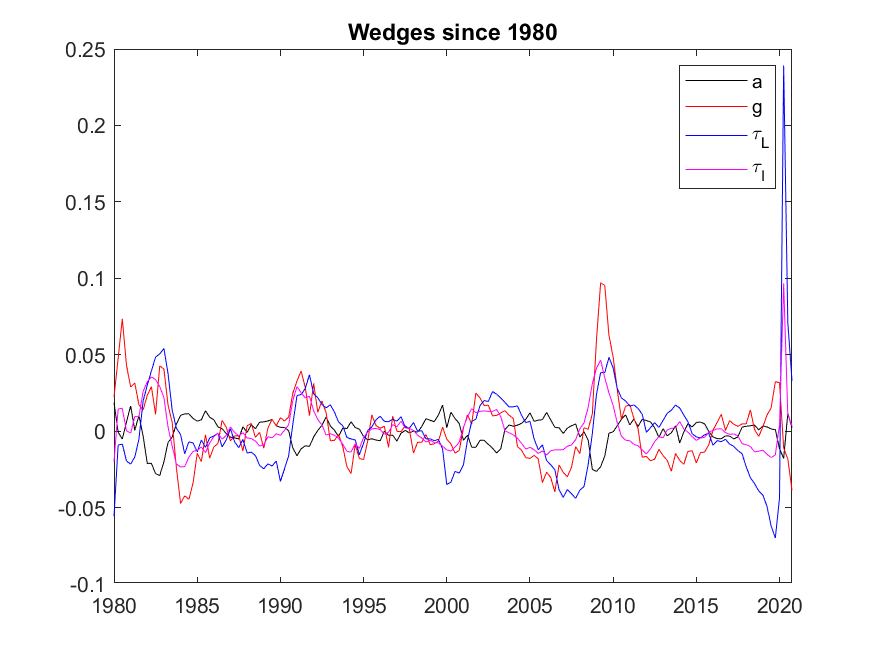
\includegraphics{wedges}

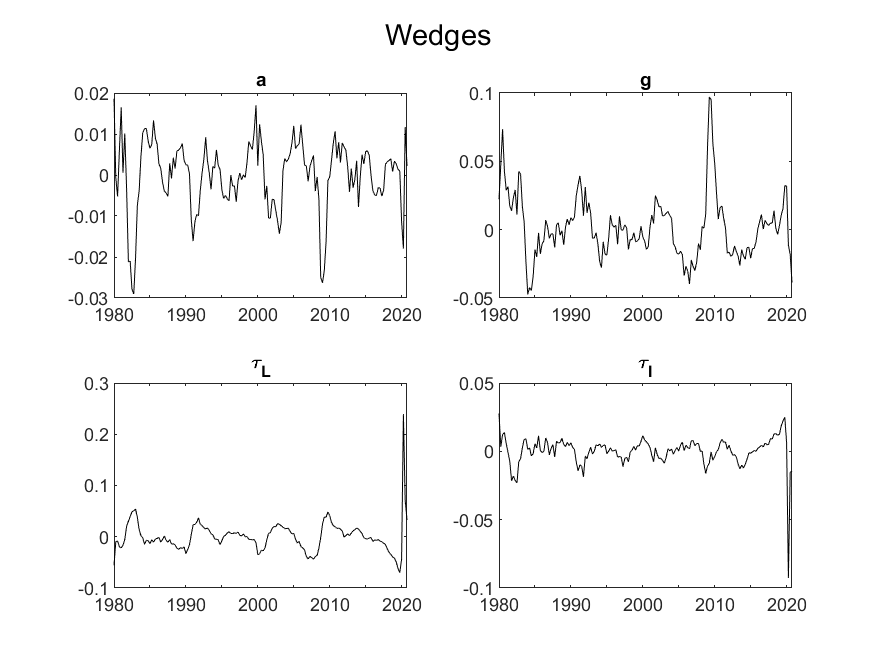
\includegraphics{wedges2}

We can now solve each model separately for each wedge and calculate GDP implied by these models. To do so, we can take advantage of the following relationship which we derived earlier:
\begin{align*}
q_{1,1}k_t + q_{1,2}c_t &= \Theta_1 a_t + \Theta_2 g_t + \Theta_3 \hat{\tau}_{L,t} + \Theta_4\hat{\tau}_{I,t}\\
\Rightarrow c_t &= \frac{-q_{1,1}k_t + \Theta Z_t }{q_{1,2}}.
\end{align*}

We calculate each period's capital by iterating forward from the law of motion of capital.

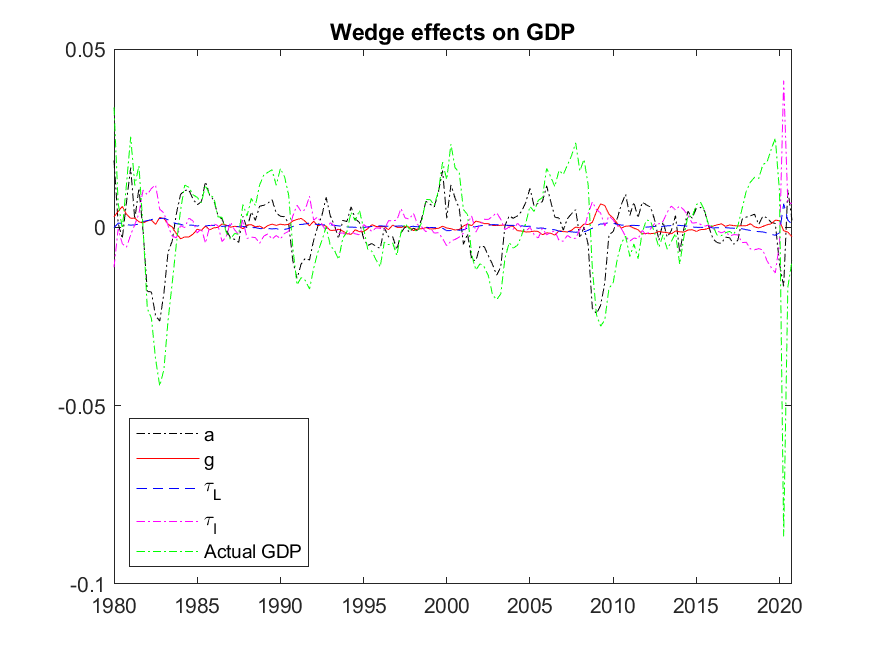
\includegraphics{wedgesg}

The above figure shows the output series counterfactuals calculated using only one shock at a time. In my opinion it appears that $\tau_L$ tracks GDP the best overall, with $a$ also tracking well pre-2005. However, $a$'s relationship to GDP seems to be less consistent post-2005. $g,\tau_{I}$ appear to be flat and counter-cyclical. In the figures to come, we will zoom in to the financial crisis of 2008 and the recent Covid pandemic.

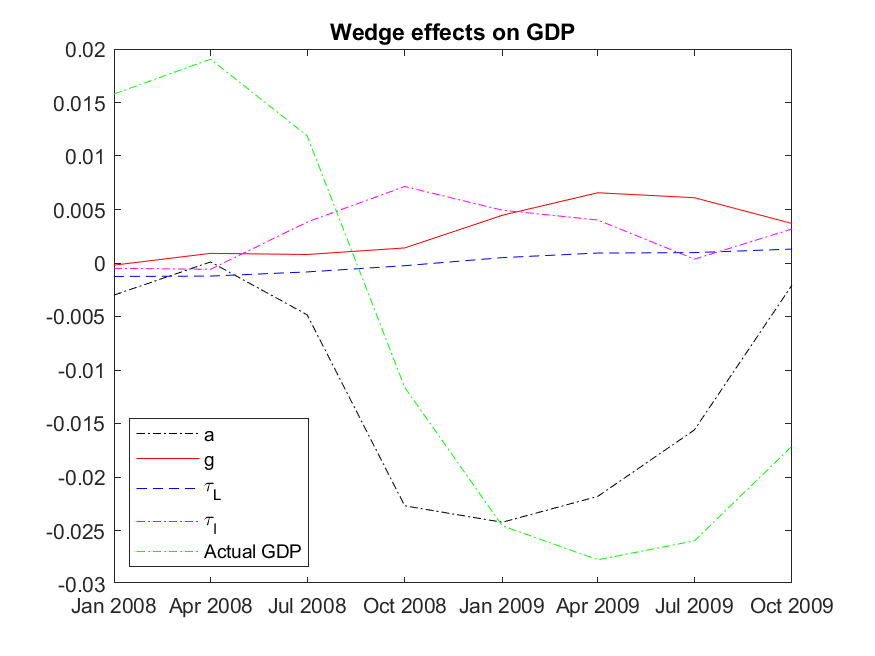
\includegraphics{wedgesfin}

The above figure shows the zoomed-in movements in the GDP implied by the various shocks surrounding the global financial crisis. What follows is a similar figure detailing the change in GDP from all shocks in the same time frame.

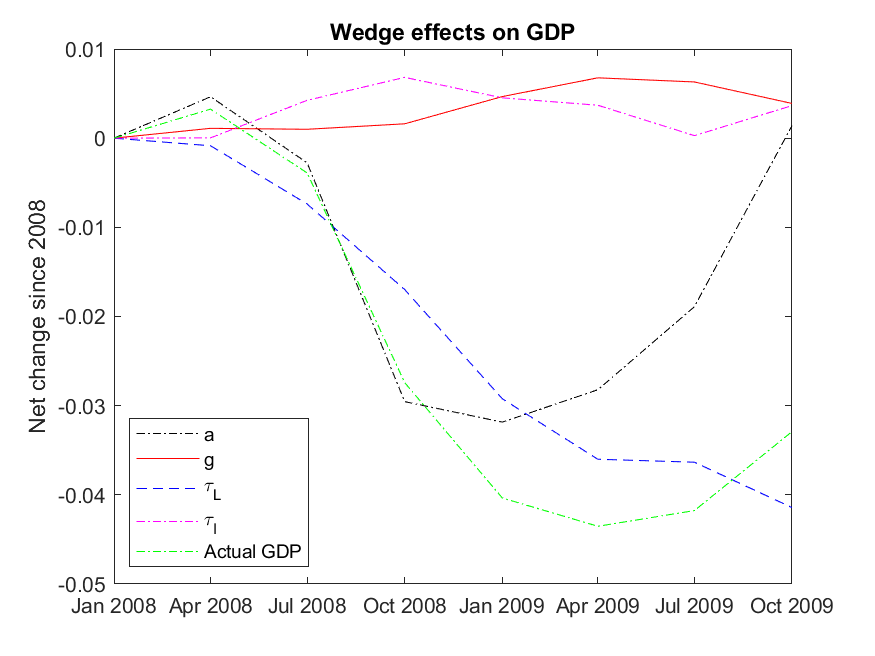
\includegraphics{wedgesfindiff}

In the above figure we can see the change from the beginning of 2008 of GDP from all of the models. $\tau_L$ appears to closely track GDP over this period, and $a$ also accounts for some of the variation in GDP. We will now move on to the Covid pandemic.

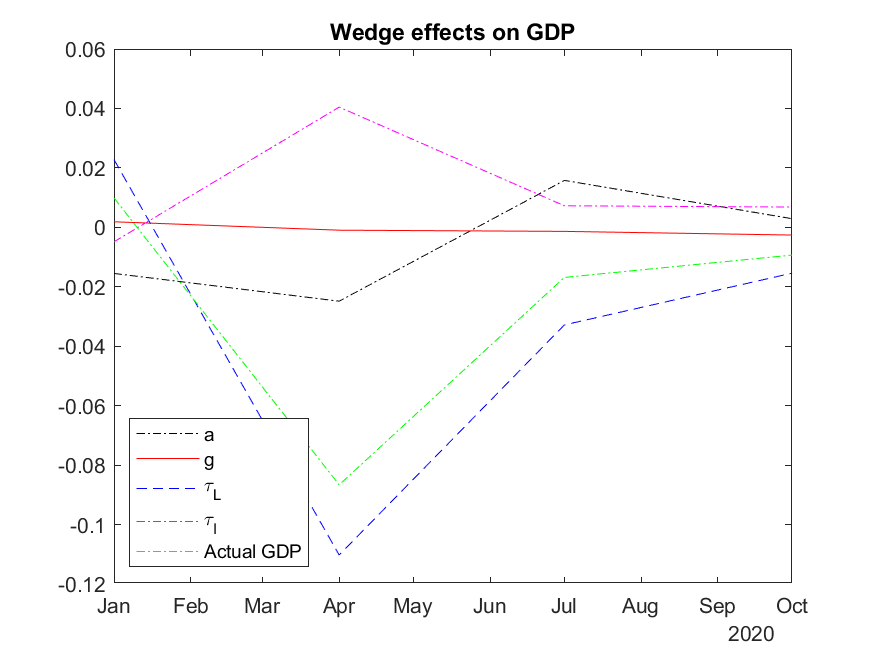
\includegraphics{wedgescov}

In the above figure, we can observe the zoomed-in movements in the GDP implied by the various shocks surrounding the Covid pandemic. What follows is a similar figure detailing the change in GDP from all shocks in the same time frame.

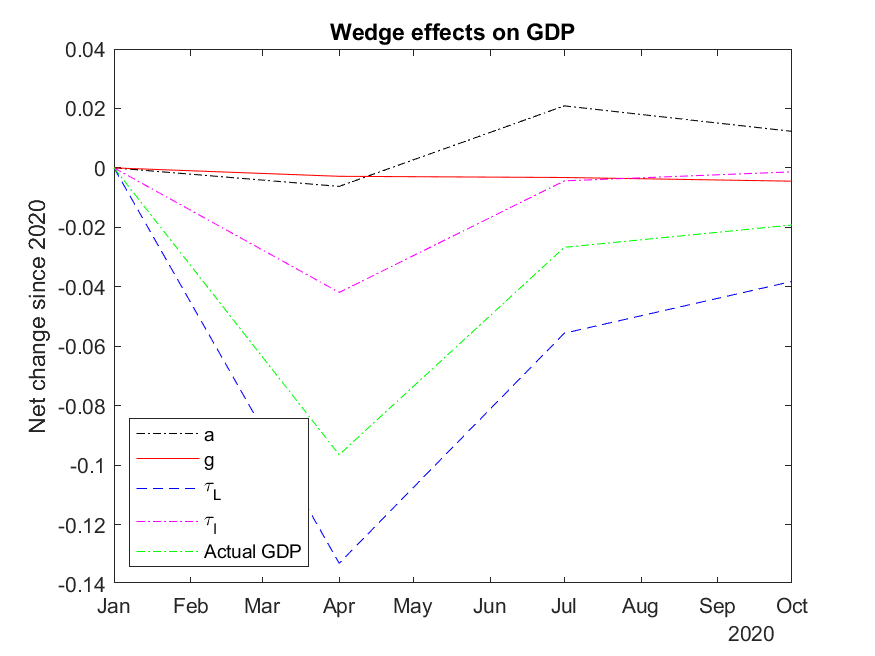
\includegraphics{wedgescovdiff}

In the above figure we can see the change from the beginning of 2020 of GDP from all of the models. $\tau_L$ appears to be the main driver during the Great Lockdown, which matches closely with intuition. Covid is clearly exogenous to the model, and caused mass unemployment over this period.

Overall, to summarize, during both recent crises it is apparent that most of the variation came from the labor wedge. The productivity wedge also appears to have played an important role during the financial crisis, but not during the Great Lockdown. 

%Overall, to summarize, during both recent crises we can see from the counterfactuals that the effect of the labor wedge is by far the most important. This is despite the financial crisis being seen as being driven by financial dynamics, which would come through in the investment wedge. 
\end{document}
